\documentclass{beamer}
\usetheme{Boadilla}

\usepackage{amsmath}
\usepackage{amsthm}
\usepackage{amssymb}
\usepackage{tikz}
\usepackage{leftindex}

\DeclareMathOperator{\st}{st}
\DeclareMathOperator{\diff}{d}

\newcommand{\ls}{\leftindex^*}

\newcommand{\NN}{\mathbb{N}}
\newcommand{\ZZ}{\mathbb{Z}}
\newcommand{\QQ}{\mathbb{Q}}
\newcommand{\RR}{\mathbb{R}}
\newcommand{\CC}{\mathbb{C}}
\newcommand{\HR}{\ls{\RR}}

\newcommand{\Ind}{\mathsf{I}}
\newcommand{\Dir}{\Ind_{\QQ}}

\newenvironment{remark}{
    \setbeamercolor{block title}{bg=orange!20, fg=orange}
    \begin{block}{Remark}}{\end{block}}

\usepackage{biblatex}
\addbibresource{references.bib}

\title[Intuition v.s. Deduction]{Intuition Mathematics v.s. Deduction Mathematics}
\subtitle{A discussion involving Infinities and Infinitesimals}
\author{Eason Shao}
\institute{St Paul's School}
\date{July 2, 2024}

\AtBeginSection[]
{
    \begin{frame}{Table of Contents}
        \tableofcontents[currentsection]
    \end{frame}
}

\begin{document}

\frame{\titlepage}

\begin{frame}{Table of Contents}
    \nocite{nsa}
    \nocite{tp}
    \nocite{hr}
    \nocite{ift}
    \nocite{calc}
    \nocite{hocalc}
    \tableofcontents
\end{frame}

\section{Calculus of Infinitesimals}

\begin{frame}{Calculus of Infinitesimals}
    \begin{itemize}
        \onslide<+->{\item c. 1660, Newton, Leibnitz: Formulation of Non-rigorous Calculus with Infinitesimals.}

              \onslide<+-> {\begin{example}
                  They argue that the derivative of \(f(x) = x^2\) is \(f'(x) = 2x\), since}
                  \begin{align*}
                      \onslide<+->{f'(x) & = \frac{f(x + o) - f(x)}{o}\\}
                      \onslide<+->{      & = \frac{(x + o)^2 - x^2}{o}\\}
                      \onslide<+->{      & = \frac{2 x o + o^2}{o}\\}
                      \onslide<+->{      & = 2x + o\\}
                      \onslide<+->{      & = 2x.}
                  \end{align*}
              \end{example}

              \onslide<+->{Rating:} \onslide<+->{Deduction 1,} \onslide<+->{Intuition 5.}
    \end{itemize}
\end{frame}

\begin{frame}
    \begin{itemize}
        \item c. 1820, Cauchy, Weierstrass: Formal definition of a limit (\(\epsilon-\delta\)).\pause

              \begin{definition}[The \(\epsilon-\delta\) definition of a limit]
                  The limit of \(f(x)\) as \(x\) tends to \(c\) is A, or
                  \[
                      \lim_{x \to c} f(x) = A,
                  \]
                  if and only if, for all \(\epsilon > 0\), there exists a \(\delta > 0\), such that for all \(0 < |x - c| < \delta\), we have \(|f(x) - A| < \epsilon\).
              \end{definition}\pause

              \begin{definition}[First Principles]
                  \[f'(x) = \lim_{h \to 0} \frac{f(x+h) - f(x)}{h}.\]
              \end{definition}

              Rating: \pause Deduction 5, \pause Intuition 1.
    \end{itemize}
\end{frame}

% \begin{frame}
%     \begin{itemize}
%         \item 1934, Skolem: First development of non-standard analysis.\pause
%         \item 1948, E. Hewitt and 1955, J. Łoś: Formation of non-standard analysis.\pause
%         \item 1961, A. Robinson: A mathematical (rigorous) interpretation of continuity and infinitesimals (hyperreals) based on work by Hewitt and Łoś.
%     \end{itemize}
% \end{frame}

\section{Attempt to Include Infinities and Infinitesimals}

% \begin{frame}{Transfer Principle}
%     To develop a number system that includes infinities and infinitesimals and to make it useful (and intuitive) at the same time, we really would like as many properties to preserve from \(\mathbb{R}\) to this number set, \textbf{hyperreal numbers} \(\HR\) as possible.\pause

%     \begin{theorem}[Transfer Principle from \(\RR\) to \(\HR\)]
%         Any statement of the form "for any number \(x\) ..." that is true for the reals \(x \in \RR\) is also true for the hyperreals \(x \in \HR\).
%     \end{theorem}\pause

%     \begin{remark}
%         Statements on sets and functions might not hold since they might depend on specific properties of real numbers.
%     \end{remark}

% \end{frame}

\begin{frame}{Hyperreal Numbers (from \(\RR\) to \(\HR\))}\pause
    \begin{definition}[Hyperreal Numbers]
        The \textbf{hyperreal numbers} \(\HR\) are defined to be the real numbers \(\RR\), together with:\pause
        \begin{itemize}
            \item \textbf{Infinitesimals} which have (absolute value) smaller than any real number -- \(\omega\).\pause
            \item \textbf{Infinities} which have (absolute value) larger than any real number -- \(\epsilon\).\pause
        \end{itemize}
        We define \(\omega\) as some infinity. \(\omega > x\) for all \(x \in \RR\).\pause

        We define \(\epsilon\) as some infinitesimal. For all \(x \in \RR_{+}\), \(0 < \epsilon < x\).\pause

        \[
            \epsilon \omega = 1 \iff \frac{1}{\omega} = \epsilon
        \]
    \end{definition}
\end{frame}

% \begin{frame}
%     \begin{theorem}[Transfer Principle from \(\RR\) to \(\HR\)]
%         Any statement of the form "for any number \(x\) ..." that is true for the reals \(x \in \RR\) is also true for the hyperreals \(x \in \HR\).
%     \end{theorem}\pause

%     \begin{examples}
%         \begin{enumerate}
%             \item For any real number \(x, y \in \RR\), we have \(x + y = y + x\). (Commutativitiy of Addition over \(\RR\)).\pause

%                   This also holds for hyperreal numbers \(x, y \in \HR\). We will have \(\omega + 1 = 1 + \omega\), and things like \(\epsilon^2 + \omega  = \omega + \epsilon^2\).\pause
%             \item For any real number \(x, y, z \in \RR\), \(y, z \neq 0\), we have \(\frac{x}{y} = \frac{xz}{yz}\).\pause

%                   This also holds for hyperreal numbers \(x, y, z \in \HR\) satisfying \(y, z \neq 0\). We will have, for example,
%                   \[
%                       \frac{1}{1 + \epsilon} = \frac{1 - \epsilon}{1 - \epsilon^2}.
%                   \]
%         \end{enumerate}
%     \end{examples}
% \end{frame}

\begin{frame}{Visuallization of Hyperreals} \pause
    \begin{center}
        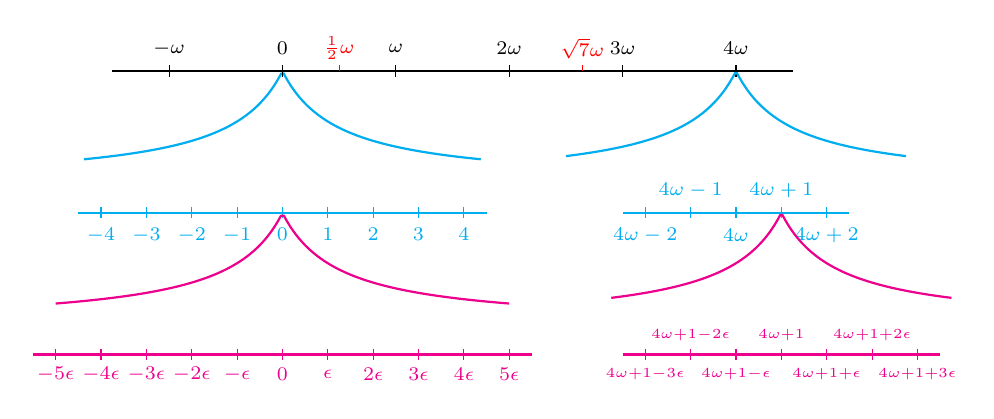
\begin{tikzpicture}[scale = 0.72]
            \onslide<+->{

                \draw [color = cyan, thick] (-3.6, 2.5) -- (3.6, 2.5);
                \foreach \x in {-4, -3, -2, -1, 0, 1, 2, 3, 4}
                \draw [color = cyan] (\x * 0.8, 2.6) -- (\x * 0.8, 2.4) node[below] {\scriptsize \(\x\)};

            }
            \onslide<+->{

                \draw[thick, magenta] plot[domain = -4:4, samples = 150] (\x,{2 / (abs(\x) + 1) + 0.5});

                \draw [color = magenta, thick] (-4.4, 0) -- (4.4, 0);
                \foreach \x in {-5, -4, -3, -2, -1, 0, 1, 2, 3, 4, 5}
                \draw [color = magenta] (\x * 0.8, 0.1) -- (\x * 0.8, -0.1);

                \foreach \x in {-5, -4, -3, -2, 2, 3, 4, 5}
                \node [color = magenta] at (\x * 0.8, -0.35) {\scriptsize \(\x\epsilon\)};

                \node [color = magenta] at  (-1 * 0.8, -0.35) {\scriptsize \(-\epsilon\)};
                \node [color = magenta] at (0 * 0.8, -0.35) {\scriptsize \(0\)};
                \node [color = magenta] at (1 * 0.8, -0.35) {\scriptsize \(\epsilon\)};

            }
            \onslide<+->{

                \draw[thick, cyan] plot[domain = -3.5:3.5, samples = 150] (\x, {2 / (abs(\x) + 1) + 3});

                \draw [thick] (-3, 5) -- (9, 5);
                \foreach \x in {-1, 0, 1, 2, 3, 4}
                \draw (\x * 2, 5.1) -- (\x * 2, 4.9);

                \foreach \x in {2, 3, 4}
                \node at (\x * 2, 5.4) {\scriptsize \(\x\omega\)};


                \node at (-2, 5.4) {\scriptsize \(-\omega\)};
                \node at (0, 5.4) {\scriptsize \(0\)};
                \node at (2, 5.4) {\scriptsize \(\omega\)};

                \draw [color = red] (1, 5.1) -- (1, 5);
                \node [color = red] at (1, 5.4) {\scriptsize \(\frac{1}{2}\omega\)};

                \draw [color = red] (5.2915026221, 5.1) -- (5.2915026221, 5);
                \node [color = red] at (5.2915026221, 5.4) {\scriptsize \(\sqrt{7}\omega\)};

            }
            \onslide<+->{

                \draw[thick, cyan] plot[domain = -3:3, samples = 150] (\x + 8, {2 / (abs(\x) + 1) + 3});

                \draw [color = cyan, thick] (6, 2.5) -- (10, 2.5);
                \foreach \x in {-2, -1, 0, 1, 2}
                \draw [color = cyan] (\x * 0.8 + 8, 2.6) -- (\x * 0.8 + 8, 2.4);


                \node [color = cyan] at (-2 * 0.8 + 8, 2.1) {\scriptsize \(4\omega - 2\)};
                \node [color = cyan] at (-1 * 0.8 + 8, 2.9) {\scriptsize \(4\omega - 1\)};
                \node [color = cyan] at (0 * 0.8 + 8, 2.1) {\scriptsize \(4\omega\)};
                \node [color = cyan] at (1 * 0.8 + 8, 2.9) {\scriptsize \(4\omega + 1\)};
                \node [color = cyan] at (2 * 0.8 + 8, 2.1) {\scriptsize \(4\omega + 2\)};

            }
            \onslide<+->{

                \draw[thick, magenta] plot[domain = -3:3, samples = 150] (\x + 8.8,{2 / (abs(\x) + 1) + 0.5});

                \draw [color = magenta, thick] (6, 0) -- (11.6, 0);
                \foreach \x in {-3, -2, -1, 0, 1, 2, 3}
                \draw [color = magenta] (\x * 0.8 + 8 + 0.8, 0.1) -- (\x * 0.8 + 8 + 0.8, -0.1);

                \node [color = magenta] at (-3 * 0.8 + 8 + 0.8, -0.35) {\(\scriptscriptstyle 4\omega + 1 - 3\epsilon\)};
                \node [color = magenta] at (-2 * 0.8 + 8 + 0.8, 0.35) {\(\scriptscriptstyle 4\omega + 1 - 2\epsilon\)};
                \node [color = magenta] at (-1 * 0.8 + 8 + 0.8, -0.35) {\(\scriptscriptstyle 4\omega + 1 - \epsilon\)};
                \node [color = magenta] at (0 * 0.8 + 8 + 0.8, 0.35) {\(\scriptscriptstyle 4\omega + 1\)};
                \node [color = magenta] at (1 * 0.8 + 8 + 0.8, -0.35) {\(\scriptscriptstyle 4\omega + 1 + \epsilon\)};
                \node [color = magenta] at (2 * 0.8 + 8 + 0.8, 0.35) {\(\scriptscriptstyle 4\omega + 1 + 2\epsilon\)};
                \node [color = magenta] at (3 * 0.8 + 8 + 0.8, -0.35) {\(\scriptscriptstyle 4\omega + 1 + 3\epsilon\)};

            }
        \end{tikzpicture}

    \end{center}
\end{frame}

\begin{frame}{Standard Part (From \(\HR\) to \(\RR\))} \pause
    \begin{definition}[Standard Part]
        If some hyperreal number \(x \in \HR\) and is finite, then we define the function \(\st\), as
        \[
            \st (x) = \text{the closest real number to \(x\)}.
        \]
    \end{definition} \pause

    \begin{examples}
        \begin{enumerate}
            \item \(\st (2 + \epsilon) = 2\), \pause
            \item \(\st (3 - \epsilon + \epsilon^4) = 3\).
        \end{enumerate}
    \end{examples}

\end{frame}

\section{What we can do with it}

\begin{frame}{Derivative}
    For a function \(f\), we defined its derivative using First Principles:
    \begin{definition}[First Principles]
        \[
            f'(x) = \lim_{h \to 0} \frac{f(x+h) - f(x)}{h}.
        \]
    \end{definition}\pause

    Here, \(h\) is just an infinitesimal, and so we can define the derivative using hyperreals as follows:
    \begin{definition}[Derivative from Hyperreals]
        \[
            f'(x) = \st\left(\frac{f(x + \epsilon) - f(x)}{\epsilon}\right).
        \]
    \end{definition}
\end{frame}

\begin{frame}
    \begin{example}
        Let us use this to find the derivative of \(f(x) = x^n\).
        \begin{align*}
            \onslide<+->{f'(x) & = \st\left(\frac{(x+\epsilon)^n - x^n}{\epsilon}\right)\\}
            \onslide<+->{      & = \st\left(\frac{\left(x^n + n \epsilon x^{n-1} + \frac{n(n-1)}{2}\epsilon^2 x^{n - 2} + \ldots\right) - x^n}{\epsilon}\right)\\}
            \onslide<+->{      & = \st\left(\frac{n \epsilon x^{n-1} + \frac{n(n-1)}{2}\epsilon^2 x^{n - 2} + \ldots}{\epsilon}\right)\\}
            \onslide<+->{      & = \st \left(n x^{n-1} + \square \epsilon\right),}
        \end{align*}

        \onslide<+->{where \(\square\) is something that is not infinity.}

        \onslide<+->{So \(\square \epsilon\) must be an infinitesimal, and the standard part of this must be \(n x^{n-1}\).}

        \onslide<+->{This is consistent with what we learned in class.}
    \end{example}
\end{frame}

\begin{frame}{Limits}
    Now we look at how we can define a limit in non-standard analysis using Hyperreals.\pause

    \begin{definition}[Limits]
        We define
        \[
            \lim_{x \to +\infty} f(x) = \st(f(\omega)), \lim_{x \to -\infty} f(x) = \st(f(-\omega)).
        \]
        and
        \[
            \lim_{x \to a^{+}} f(x) = \st(f(a + \epsilon)), \lim_{x \to a^{-}} f(x) = \st(f(a - \epsilon)).
        \]
    \end{definition}\pause

    It is soon apparent that this and the First Principle give the exact definition of the derivative.
\end{frame}

\begin{frame}
    If we recall the definition of \(e\):
    \begin{definition}[\(e\)]
        \[
            e = \lim_{x \to \infty} \left(1 + \frac{1}{x}\right)^x = \st \left(\left(1 + \frac{1}{\omega}\right)^\omega\right)  = \st \left(\left(1 + \epsilon\right)^\omega\right),
        \]
    \end{definition}
    we try to find the derivative of \(g(x) = e^x\).\pause

    \begin{example}
        \begin{align*}
            \onslide<+->{g'(x) & = \st \left(\frac{e^{x + \epsilon} - e^x}{\epsilon}\right)
                = e^x \st \left(\frac{e^\epsilon - 1}{\epsilon}\right)\\}
            \onslide<+->{      & = e^x \st \left(\frac{\left(1 + \epsilon \right)^{\omega\epsilon} - 1}{\epsilon}\right)\\}
            \onslide<+->{      & = e^x \st \left(\frac{1 + \epsilon - 1}{\epsilon}\right)\\}
            \onslide<+->{      & = e^x \st \left(1\right)\\}
            \onslide<+->{      & = e^x.}
        \end{align*}
    \end{example}
\end{frame}

\section{Limitation}

\begin{frame}{Limitation}
    There is a famous function called the \textbf{Dirichlet Function}, which is not continuous at any point.\pause

    \begin{definition}[Dirichlet Fucntion]
        The \textbf{Dirichlet Function} \(\Dir: \RR \to \{0, 1\}\) is defined as
        \[
            \Dir(x) = \begin{cases}
                1, & x \in \QQ,               \\
                0, & x \in \RR \setminus \QQ.
            \end{cases}
        \]
    \end{definition} \pause

    It is difficult to formalize this function using hyperreals intuitively since we did not classify hyperreals as rational and irrational \pause -- things like \(\Dir(\epsilon)\) are not defined.
\end{frame}

\begin{frame}{But Wait ...} \pause

    Why was it okay for us to so naturally continuate a function from the real numbers \(\RR\) to the hyperreal numbers \(\HR\)? \pause (Dirchlet!) \pause

    Do improper integrals still work? \pause (How to integrate to \(\omega\)? \pause Or \(2\omega\)?)\pause

    \vspace{1pt}

    \large

    Why was it okay for us to assume that we can introduce new numbers that fits well into ordering of real numbers \(\RR\)? \pause \normalsize (Complex Numbers!) \pause

    \vspace{1pt}

    \large

    Why was it okay for us to say \(1 + \epsilon - 1 = \epsilon + 1 - 1 = \epsilon\)? \pause \normalsize (Matrix Multiplication!) \pause

    \vspace{1pt}

    \large

    Will special properties on real numbers \(\RR\), such as the intermediate value theorem, still hold on hyperreals \(\HR\)? \pause \normalsize (Rationals!) \pause

    \vspace{1pt}

    \Large

    Why is it okay for us to just introduce a whole new set of numbers that seem to behave like, and yet aren't reals? \pause

    \normalsize
    (Why aren't they included in the first place?) \pause

    \vspace{1pt}

    \LARGE How can we just take this for granted?
\end{frame}

\begin{frame}{References}
    \printbibliography
\end{frame}

\end{document}